
\chapter{基于波动随机照明的透过散射介质超光学记忆效应范围成像}

非侵入式光学成像在从生物成像技术\cite{zhao_non-invasive_2001,artzi_vivo_2011}到光学检测\cite{kozloff_non-invasive_2009}的各个领域都有重要应用。但是,不均匀的样品(例如生物组织)会散射光,从而导致探测器上出现复杂的散斑图案\cite{Goodman1976,Bender}。
随着穿透深度的增加,从散射光中分离出少量的弹道光成为一个很大的挑战\cite{Abramson1978,huang_optical_1991}。多年来,人们提出了许多方法来通过利用或抑制散射光来克服透过散射介质实现非入侵成像的问题。随着空间光调制器的发展,许多方法已经被提出实现控制和操纵散射光的方法\cite{Mosk2012,rotter_light_2017}。目前,已经提出了几种技术来通过使用反馈信号来优化入射光波前来实现聚焦,以重新形成一个焦点,然后利用扫描的方式实现成像\cite{Vellekoop2007,Horstmeyer2015}。这些技术通常需要途径至散射层的两侧获取信号以优化波前,这些条件极大地限制了它们在实际场景中的应用。
为了克服这个问题,已经提出了基于波前整形和各种反馈信号(例如荧光或超声信号)的其他策略\cite{Horstmeyer2015,Katz2019,Popoff2010,Hofer2019},实现波前整形。然而,这些方法要么需要较长的采集时间,要么仅限于小视场 。
另一方面,还提出了几种利用角散斑相关性的技术\cite{bertolotti_non-invasive_2012,katz_non-invasive_2014},即光学记忆效应\cite{Freund1988,Yllmaz2019,Osnabrugge},用于对隐藏在散射介质后面的物体进行成像。这些方法计算散斑图案的自相关,其本质上利用散斑的自相关与隐藏目标的自相关相同,并使用相位检索算法从自相关重建对象图像。虽然这些方法速度很快,但它们的成像范围仍然受到光学记忆效应范围的限制。前面章节中,我们对基于光学记忆效应下的散斑成像进行了原理介绍和实验验证。

线性荧光广泛应用于生物学和生物医学科学\cite{Ruan2020,Lichtman2005,mangeat_super_resolved_2021}。 它能够对细胞、亚细胞或分子成分进行成像,并具有空间分辨率高、对比度高、速度快的优点。近年来,许多技术允许使用荧光通过散射介质进行聚焦和成像。
即便如此,这些方法要么依赖于引导星 \cite{Hhorstmeyer} 的使用,仅限于光学记忆效应范围 \cite{hofer_wide_2018},要么需要表征散射介质 \cite{boniface_non_invasive_2020}。

在本章,我们提出了一种新型的成像方法,该方法使用简单地利用旋转漫射器生成的波动随机散斑照明,允许透过散射介质在一定深度上远远超出光学记忆效应范围的进行非侵入性成像。当随机照明散斑产生后,每个荧光发射器都会在探测器上产生独特的散斑图案,我们称其为“散斑指纹”。相机所捕获的每张图像都是来自不同荧光发射器的所产生的散斑指纹的非相干总和。当随机照明随着旋转器改变时,探测器上所接收的散斑的各个散斑指纹的权重随之改变。为了检索每个单独的指纹,我们在随机改变光照的同时捕获一组图像,并使用非负矩阵分解 (Non-negative Matrix Factorization,NMF) 算法对采集的数据进行去混叠。随后,通过探索指纹之间的相关性,使用指纹重建最终图像。为了验证该技术的有效性,我们通过实验证明了我们在荧光珠和连续荧光物体上的非侵入性成像方法。

\section{基于波动随机照明的透过散射介质超光学记忆效应范围成像基本原理}

\begin{figure}[htp]
	\centering
	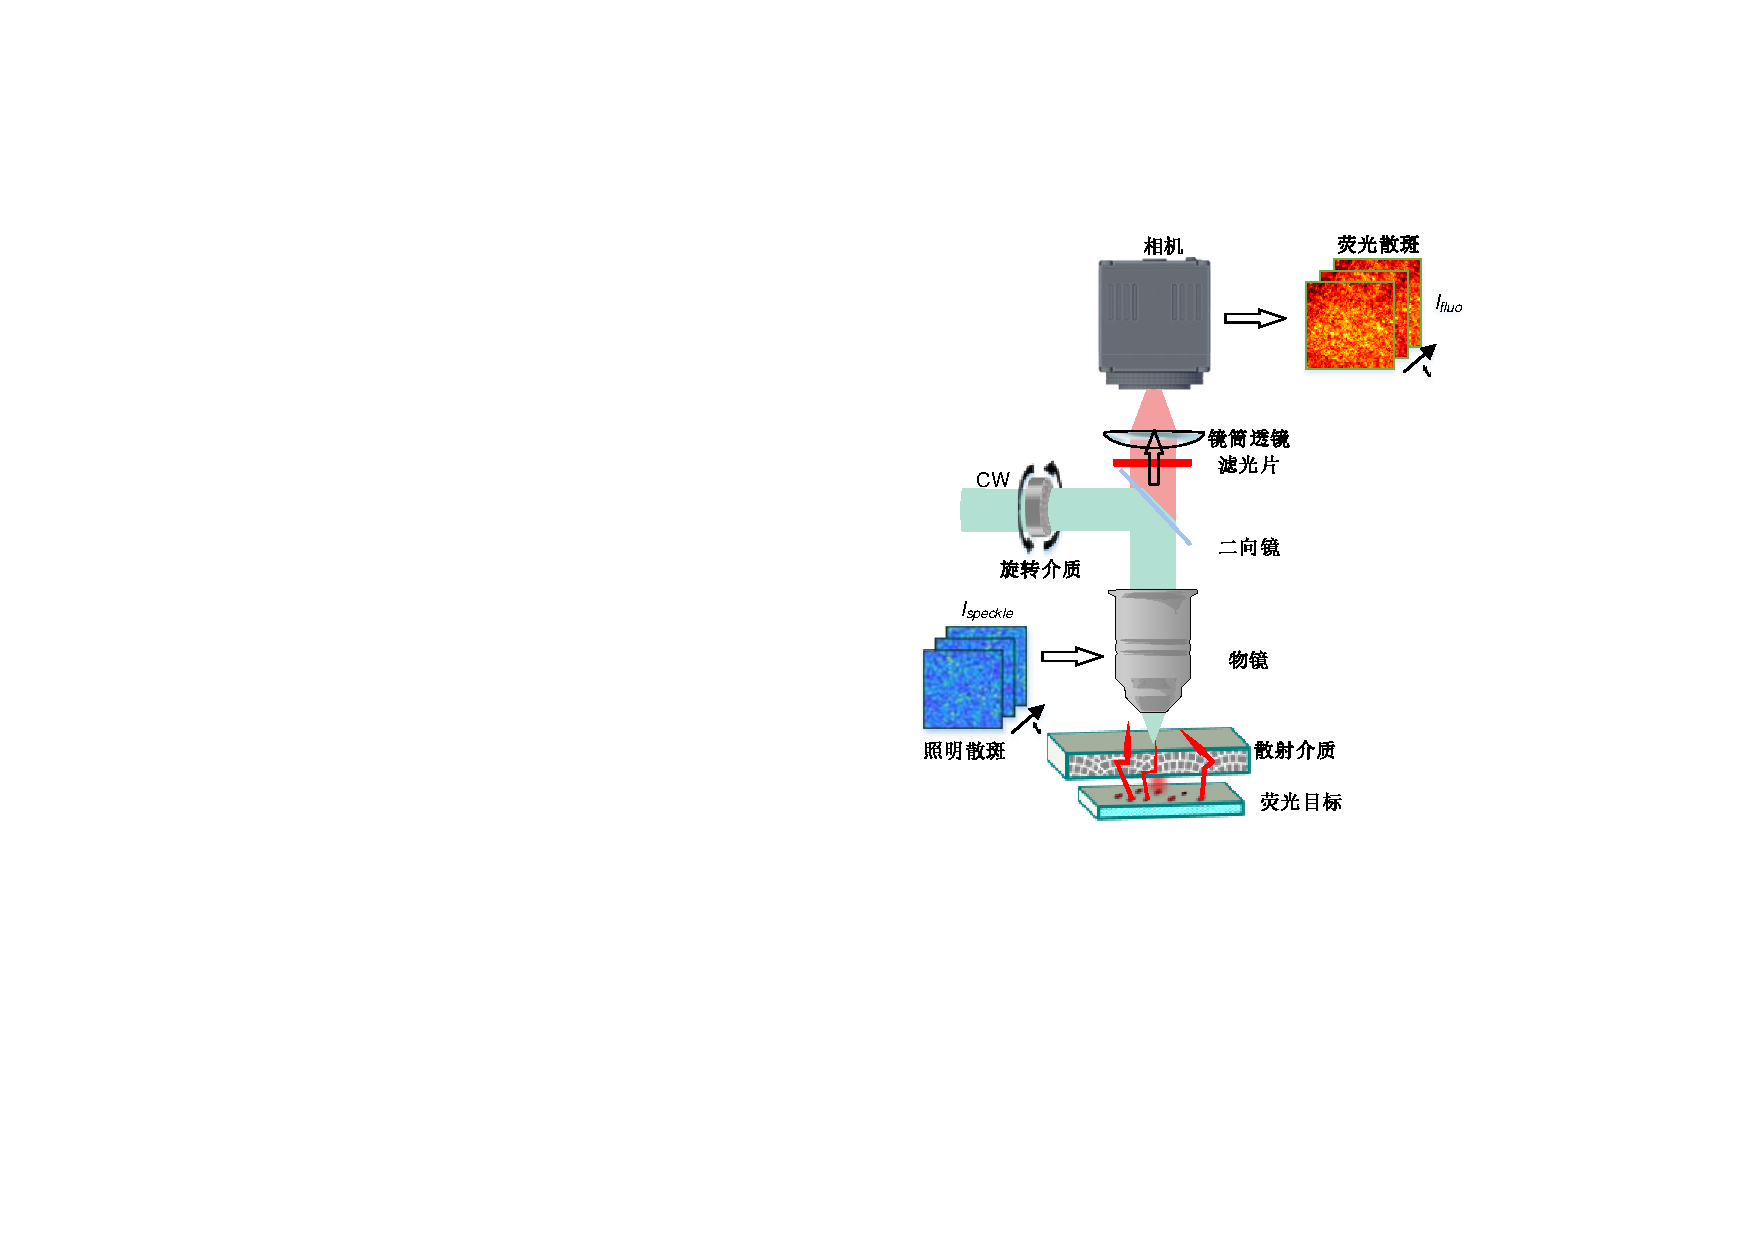
\includegraphics[scale=0.75]{C5.fig1}
	\caption{非入侵成像系统示意图}
	\label{fig:5.1}
\end{figure}

非入侵成像系统如图\ref{fig:5.1}所示。当激光通过旋转漫反射器时,入射激光被添加了随机相位实现了入射激光的随机调制,进而调制光透过散射介质产生了未知的随机散斑,未知的散斑照明目标。利用随机散斑照明目标后,目标产生自身的激发光,激发光传播并通过散射介质,产生散斑最终被相机所接收,此时相机所获得的散斑为不同散斑指纹的非相干总和。尽管捕获的图像对比度低、随机且看似无信息,但它们包含来自对象独立发射器的所有散斑指纹,且其各自的权重随着随机照明的改变具有时间的多样性。此外,光学记忆效应范围内的独立发射器将在相机上产生相关但平移的散斑指纹 \cite{Freund1988},而光学记忆效应范围外的发射器将产生完全不相关的散斑指纹。对于给定的散斑照明,捕获的图像 $I_{\textsl{fluo}}$ 可以表示为具有不同权重的散斑指纹的线性叠加。因此,相机图像$I_{\textsl{fluo}}$由下式给出:

\begin{equation}
\begin{aligned}
I_{fluo}(r,t) = \sum^{P}_{k=1} w_{k}(r) h_{k}(t),
\label{eq:5.1}
\end{aligned}
\end{equation}
其中, $I_{fluo}(r,t)$为对应于第$t$次照明时相机所接收到低对比度散斑,$r$为空间坐标,$w_{k}(r)$为第$k$个独立发射器所对应的散斑指纹,$h_{k}(t)$为第$t$次照明时第$k$个独立发射器所接收到的激光光的强度,$P$为系统中独立发射器的数量。

当拥有足够多的随机散斑照明时,就可以采集到足够的低对比度散斑图案,通过NNF对散斑集进行去混叠,获得各自发射器的散斑指纹。然后利用,指纹重建算法实现最终图像的重建。整体流程下所示;
\begin{algorithm2e}[h!]
\DontPrintSemicolon
\SetAlgoLined
\KwInput{系列散斑图案, $I_{fluo}(r,t)$.}
\KwOutput{隐藏目标的图像, $O^{Global}$.}
从系列数据集$I_{fluo}(r,t)$估计系统的秩($\rho$).\;

通过去混叠算法恢复散斑指纹($w_{i}$).\;

\For{$k=1,...,\rho$}{
在指纹$w_{k}$和其余所有的指纹($w_{i\neq k}$)之间进行成对去卷积运算.\;

获取位于与散斑指纹$w_{k}$所对应的独立发射器同一光学记忆效应范围内的独立发射器之间的相对位置.\;

获得局部重建结果($O_{k}$).\;
}

将不同区域的局部重建结果($O_{k}$)合成全局重建结果($O^{Global}$).\;

\caption{非入侵图像重建流程}
\label{alg:a1}
\end{algorithm2e}

\subsection{散斑指纹去混叠}

\begin{figure}[htp]
	\centering
	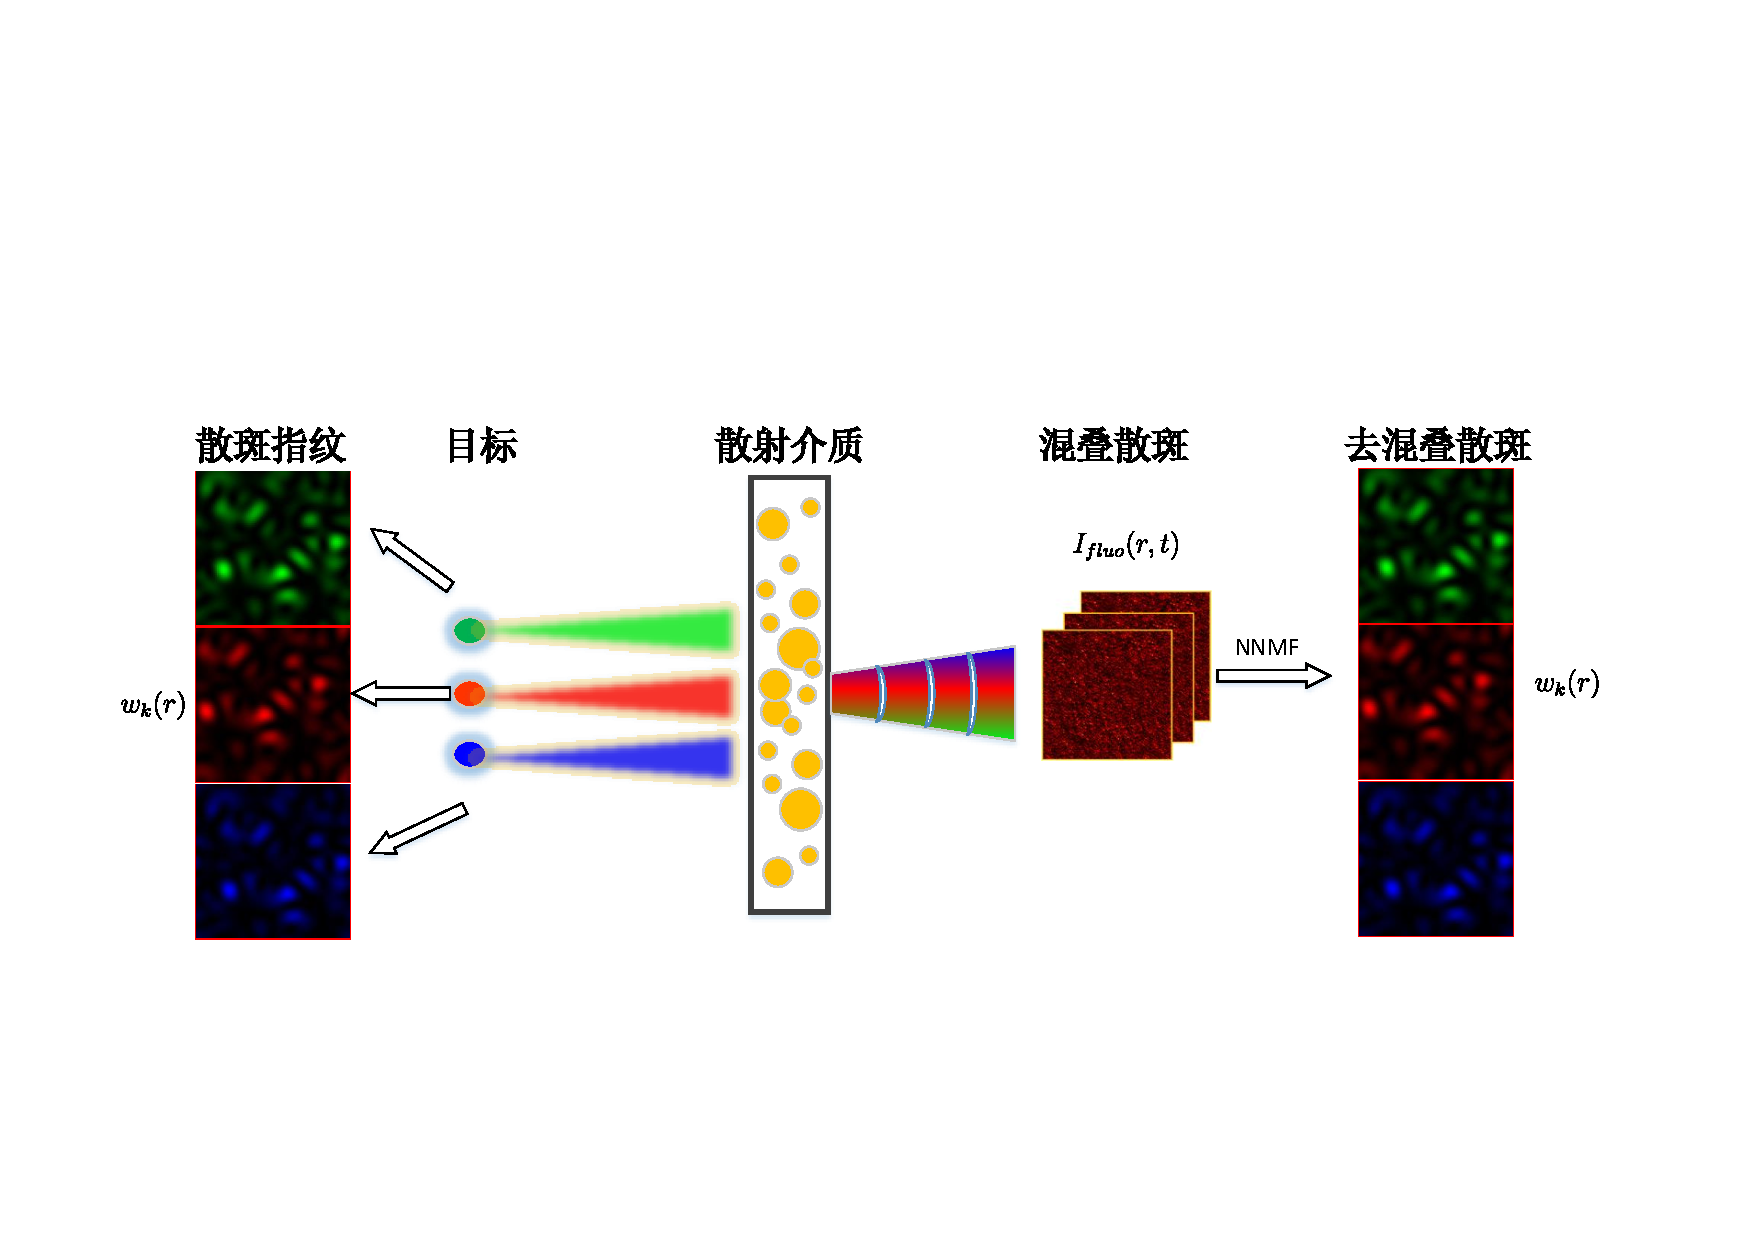
\includegraphics[scale=0.5]{C5.fig4}
	\caption{散斑去混叠示意图}
	\label{fig:5.4}
\end{figure}

如图\ref{fig:5.4}所示,独立发射器所对应的各自的散斑指纹一定,当我们使用散斑照明时,获得一些列混叠散斑。如何从一些混叠散斑中恢复出每个独立发射器的散斑指纹,将在接下来部分描述。

如公式(\ref{eq:5.1})所示,当使用随机照明时,$h_{k}(t)$随着照明的改变该随之变化。因为照明强度和散斑指纹的非负性,我们可以通过非线性优化的方式求得$w_{k}(r)$,即:

\begin{equation}
	\begin{aligned}
\min_{W>0,H>0} \Arrowvert I -WH\Arrowvert_F^{2},
\label{eq:5.2}
\end{aligned}
\end{equation}
其中,$\vert\vert M\vert\vert_F = \sqrt{\sum_i\sum_j \vert M_{ij}\vert^2}$为Frobenius矩阵范数。公式(\ref{eq:5.2})最小化问题可以表述为一个低秩分解问题。$I \in \mathbb{R}_{+}^{r \times t} $包含所有的散斑图案$I_{fluo}(r,t)$,$I \in \mathbb{R}_{+}^{r \times t}$ 可以被近似为两个实数矩阵$W \in \mathbb{R}_{+}^{r \times \rho}$ 和$H \in \mathbb{R}_{+}^{\rho \times t}$。
矩阵$W \in \mathbb{R}_{+}^{r \times \rho}$为指纹矩阵,$H \in \mathbb{R}_{+}^{\rho \times t}$为时间矩阵,其中 $r$ 是像素,$\rho$ 是 $I$矩阵所估计的秩,$t$ 表示散斑帧数。由于收集到的图像和混合指纹都具有非负性,这个问题正好对应于NMF优化问题。
NMF算法常用于去混叠场景,例如结构性成像\cite{boniface_non_invasive_2020}和功能性成像\cite{Moretti2020a,Pegard2016, Pnevmatikakis2016}等,NMF去混叠过程如图\ref{fig:5.2}所示。
在数据矩阵去混叠之前,我们需要对所获得的相机散斑进行滤波,去除散斑的轮廓噪声,在傅里叶域中移除低频信号,如图\ref{fig:5.3}所示。即在在NMF算法的运行过程前,我们需要确定$\rho$,该参数可以通过最小化NMF的均方根残差作为秩的函数来从数据中估计。

\begin{figure}[htp]
	\centering
	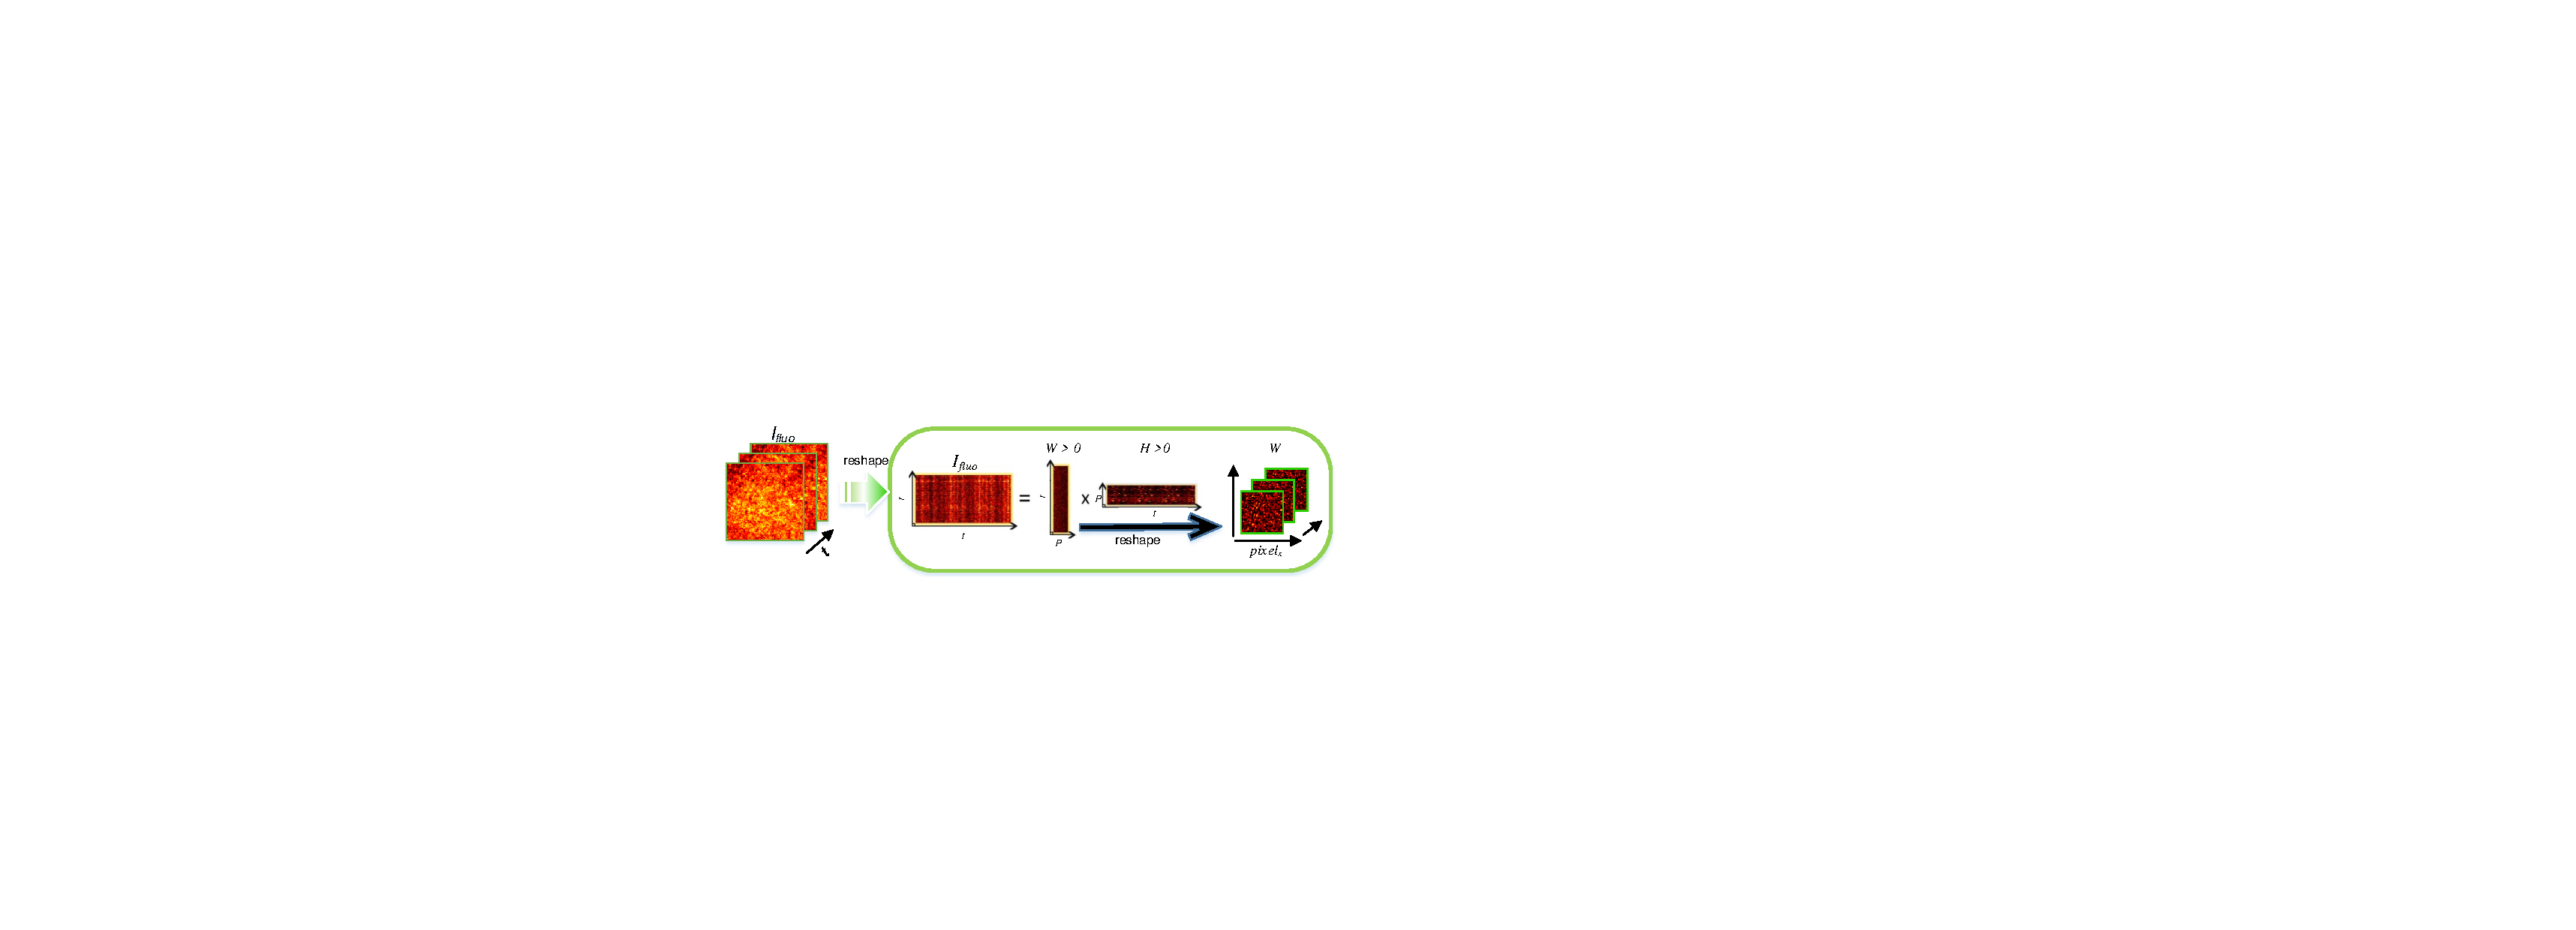
\includegraphics[scale=1.0]{C5.fig2}
	\caption{散斑指纹去混叠过程}
	\label{fig:5.2}
\end{figure}

\begin{figure}[htp]
	\centering
	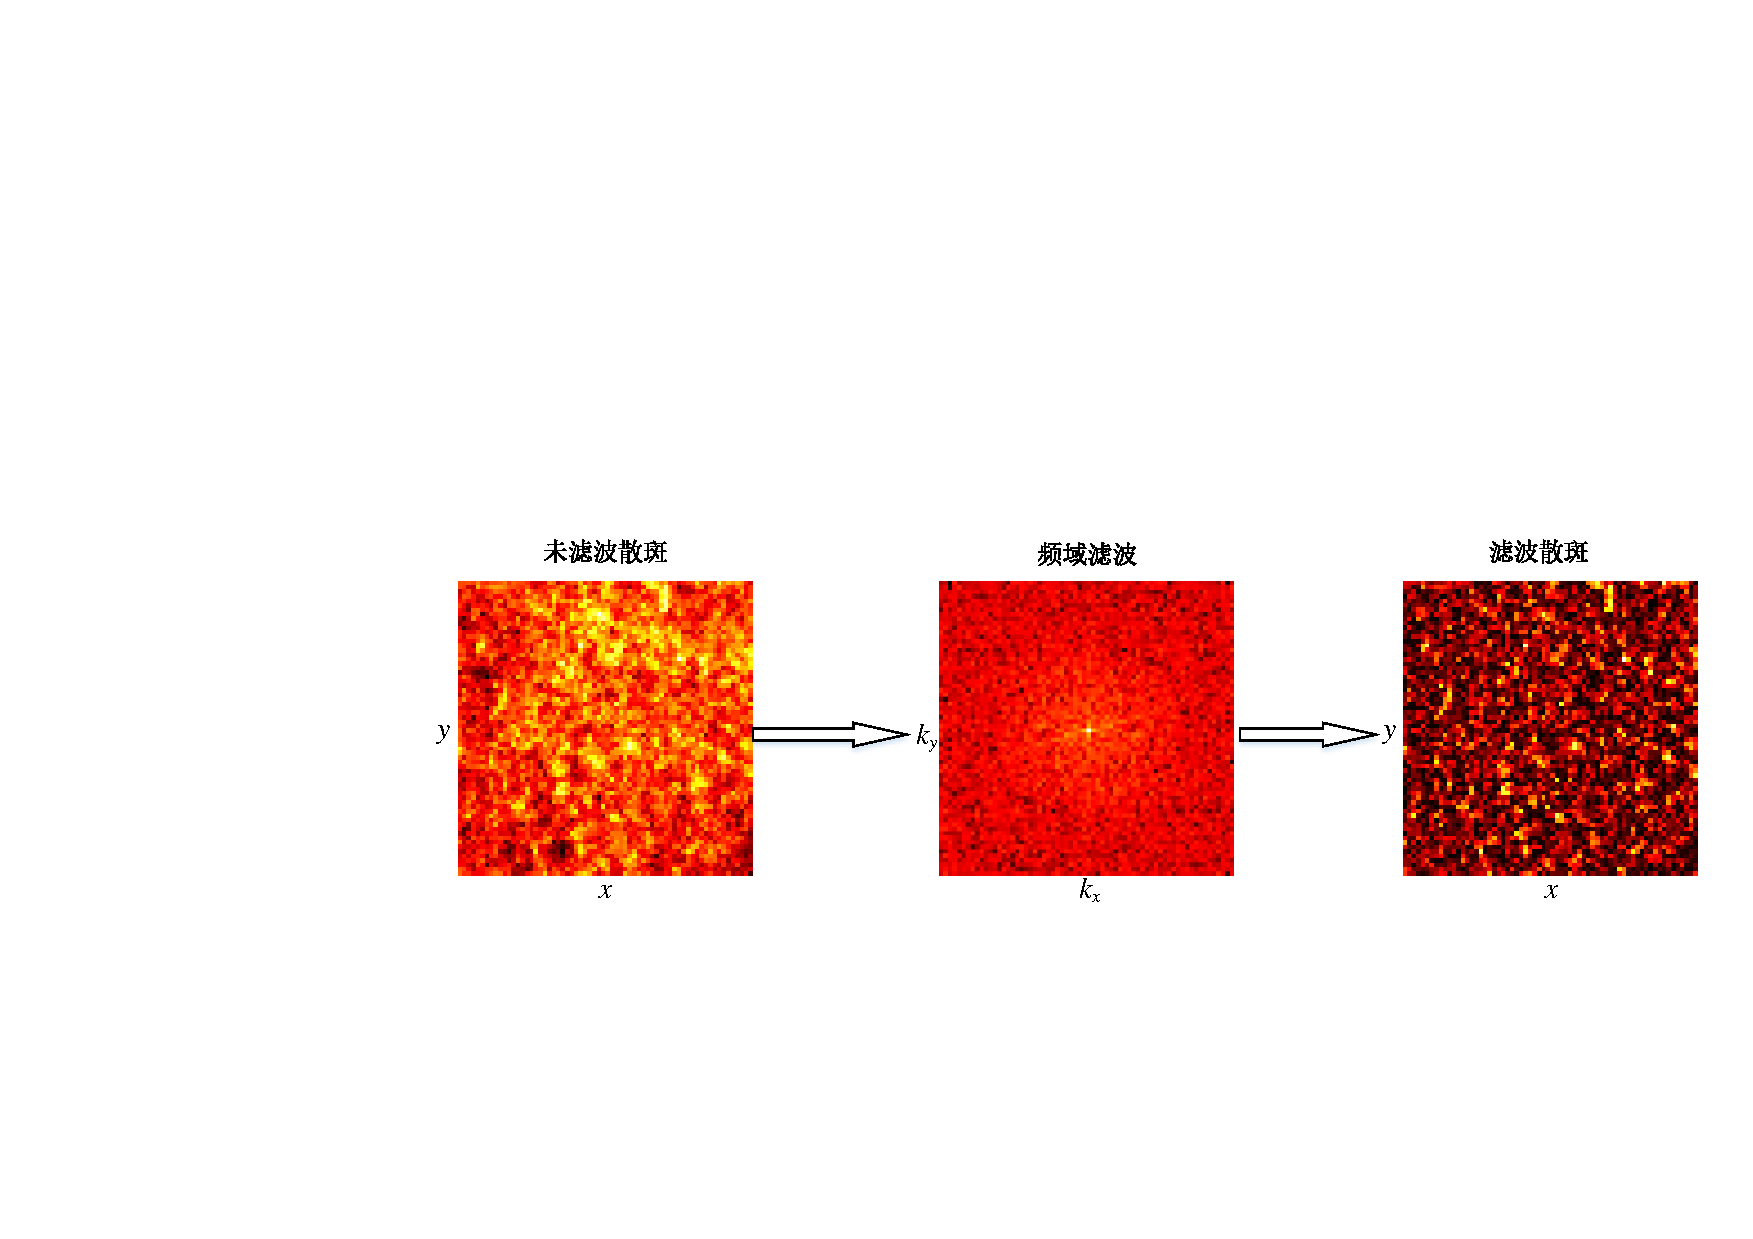
\includegraphics[scale=0.5]{C5.fig3}
	\caption{散斑滤波}
	\label{fig:5.3}
\end{figure}

为了运行NMF算法,矩阵秩$\rho$是一个需要预先确定的唯一参数。通常可以使用几种方法来估计$\rho$,例如使用 \textsl{k}-means 算法 \cite{Moretti2020a} 查看集群的数量,或者通过估计损失函数的“拐点”\cite{boniface_non_invasive_2020,hutchins_position_dependent_2008}。
在我们的使用情境下,为了简化该估计过程,我们尝试不同的数值作为该矩阵的$\rho$,记录不同数值所对应的均方根残差(Root Mean Square Residual,RMSR):$\vert\vert I_{fluo}-WH \vert\vert_{Fro}$。然后,RMSR最小值所对应的$\rho$,即该值为系统的秩$\rho$。为了验证我们所提出方法的有效性,于是进行了相应的仿真,仿真结果如图\ref{fig:5.5}所示。首先,我们生成5个点源目标,利用卷积模型生成各自的散斑指纹,并采用随机照明的方式对目标机型照明,记录其相应的散斑图案。然后根据前面所描述的矩阵秩$\rho$估计方法进行估计。图\ref{fig:5.5}中,三角形符号指示出RMSR的最小值,实线代表12次均方根值的平均值,每次的NMF优化采用不同的随机初始值。
三角形符号表示RMSR的最小均值,实线代表12次均方根值与NMF随机初始化值的均值,星号是误差条,表示其正负方向的标准偏差。通过仿真可至,当估计的秩$\rho$ 等于系统的真实秩$P$ 时,平均RMSR值为最小。我们同时分别尝试了,不同数量的点源目标,仿真结果如图\ref{fig:5.5}所示。其仿真结果表明:RMSR的最小值分别为:5,10和15,与真实值非常吻合。

\begin{figure}[htp]
	\centering
	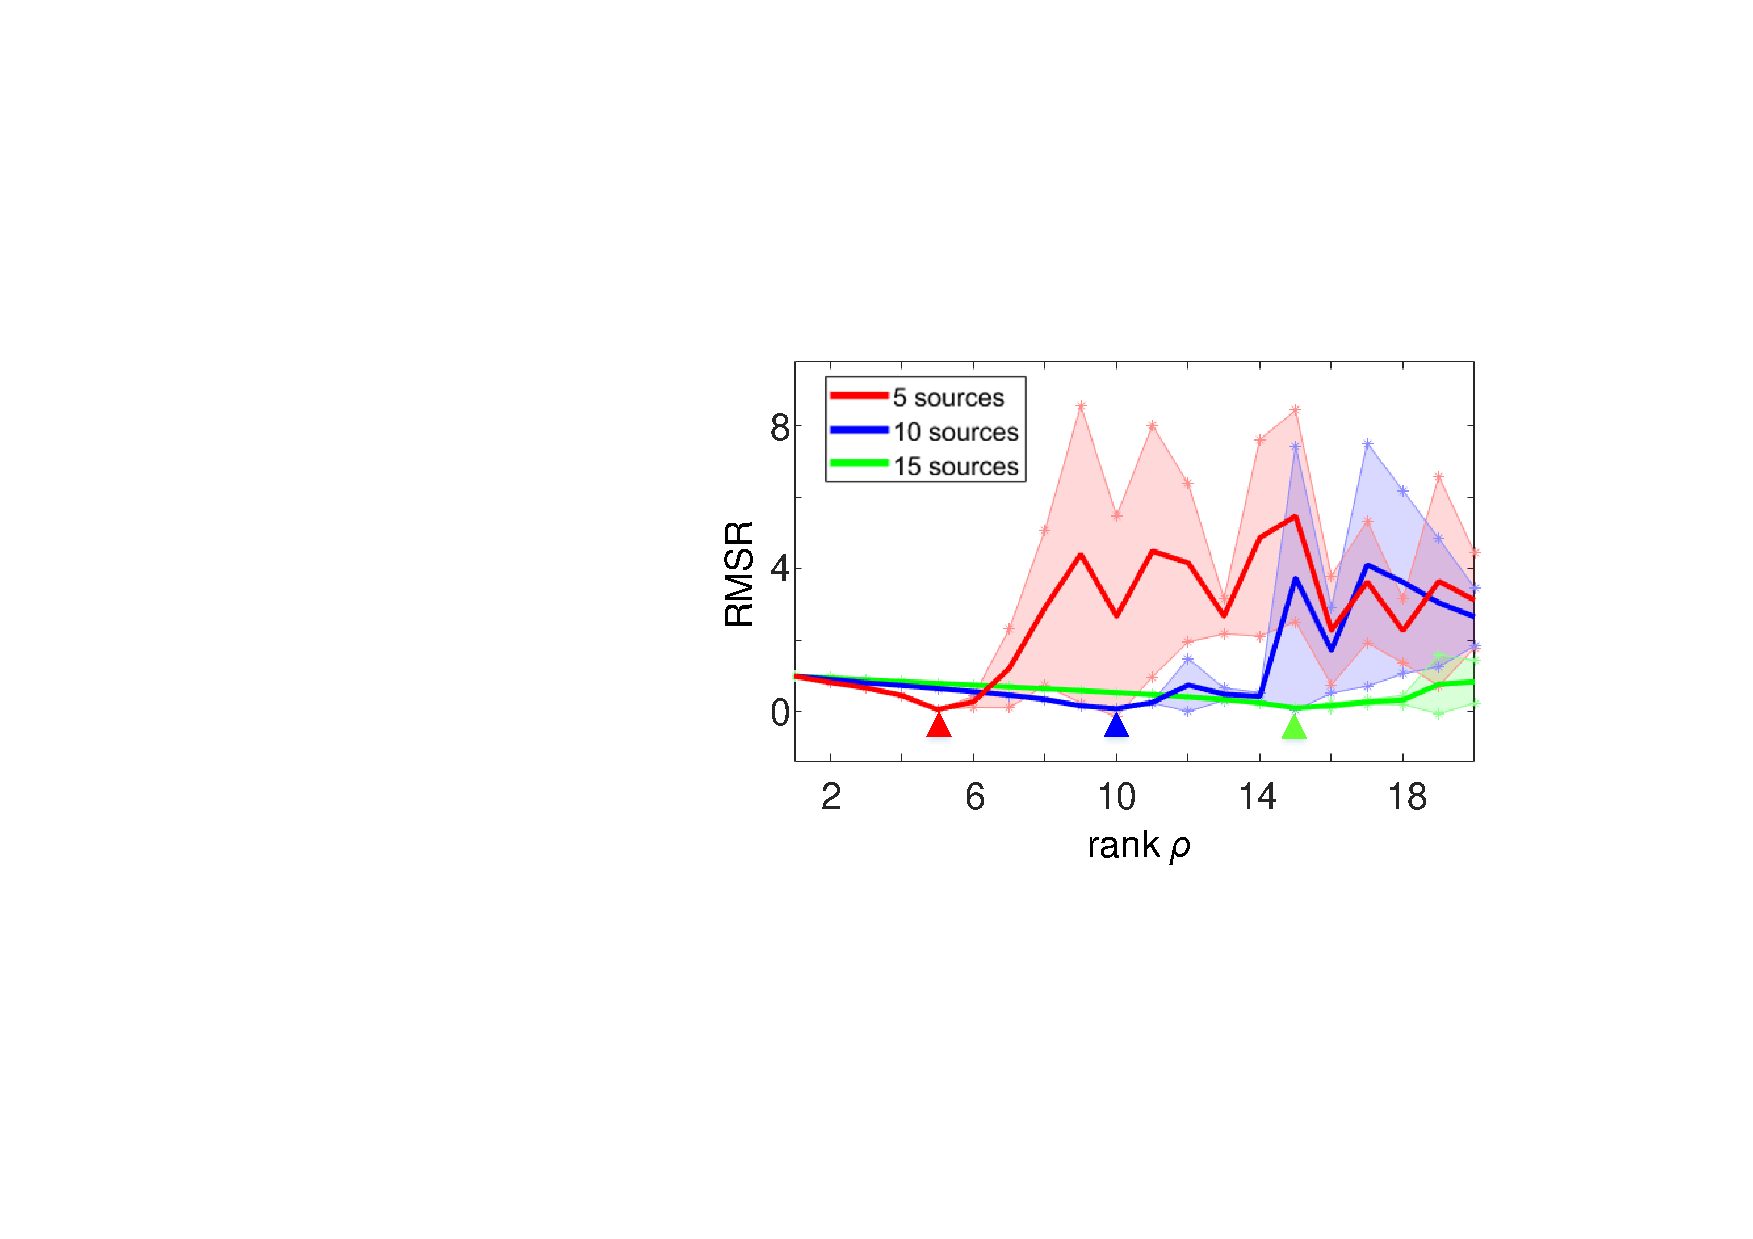
\includegraphics[scale=0.5]{C5.fig5}
	\caption{系统的秩$\rho$估计(仿真)}
	\label{fig:5.5}
\end{figure}

此外,我们通过实验证明该了估计方法的有效性。在实验中,通过随机放置11荧光珠为目标,利用旋转毛玻璃提供随机照明,记录其荧光散斑图案,并进行该数据集秩的估计,实验结果如图\ref{fig:5.6}所示。如图\ref{fig:5.6}(b)所示,所估计的$\rho$与系统真实$P$保持一致。同时,我们还在\ref{fig:5.6}(a)中提前展示了其图像的重建结果,左图为真实目标,右图为重建结果。通过仿真和实验的方式,证明了估计数据集秩的方法有效性。

\begin{figure}[htp]
	\centering
	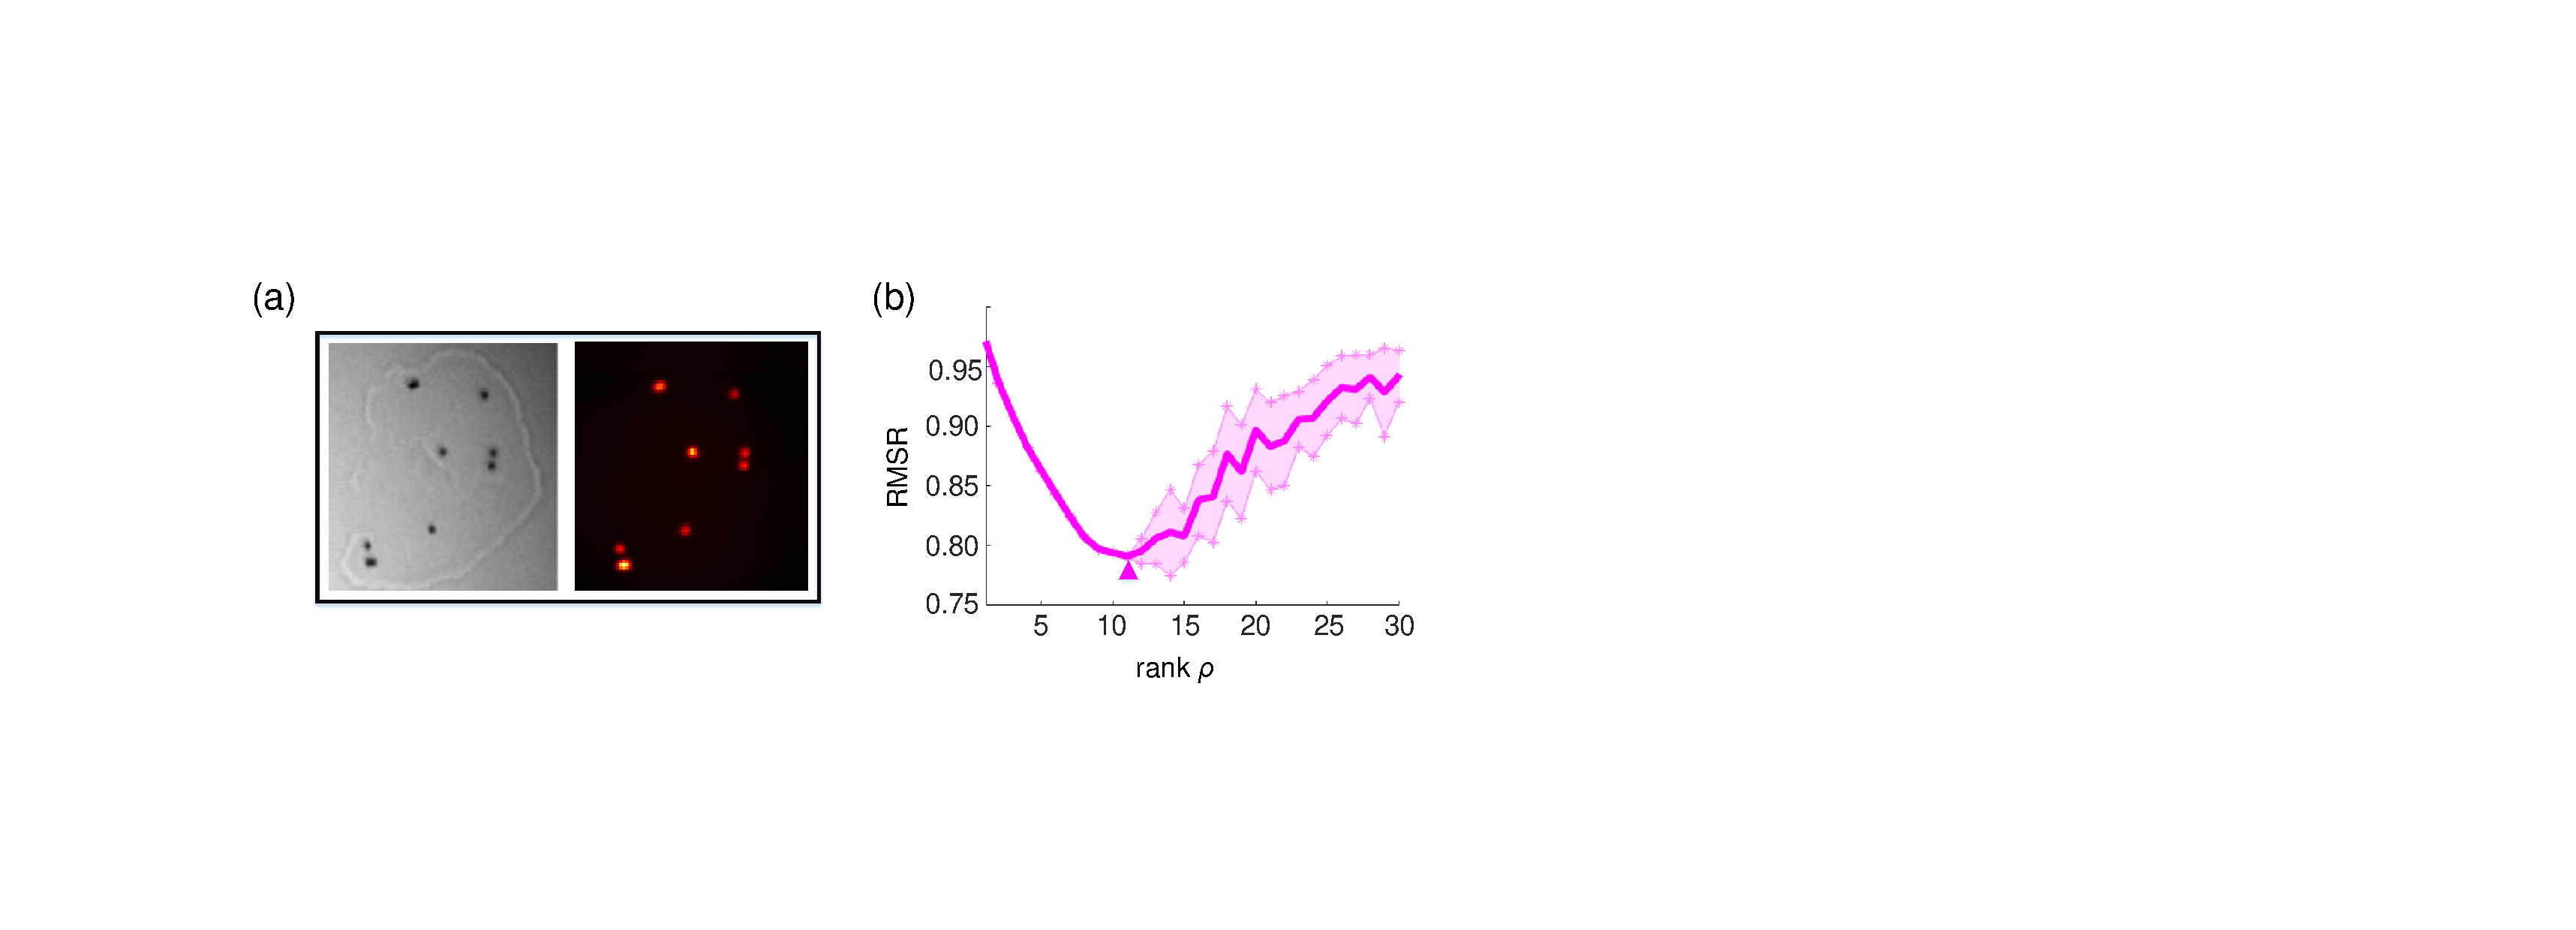
\includegraphics[scale=0.5]{C5.fig6}
	\caption{系统的秩$\rho$估计(实验)}
	\label{fig:5.6}
\end{figure}

\begin{figure}[htp]
	\centering
	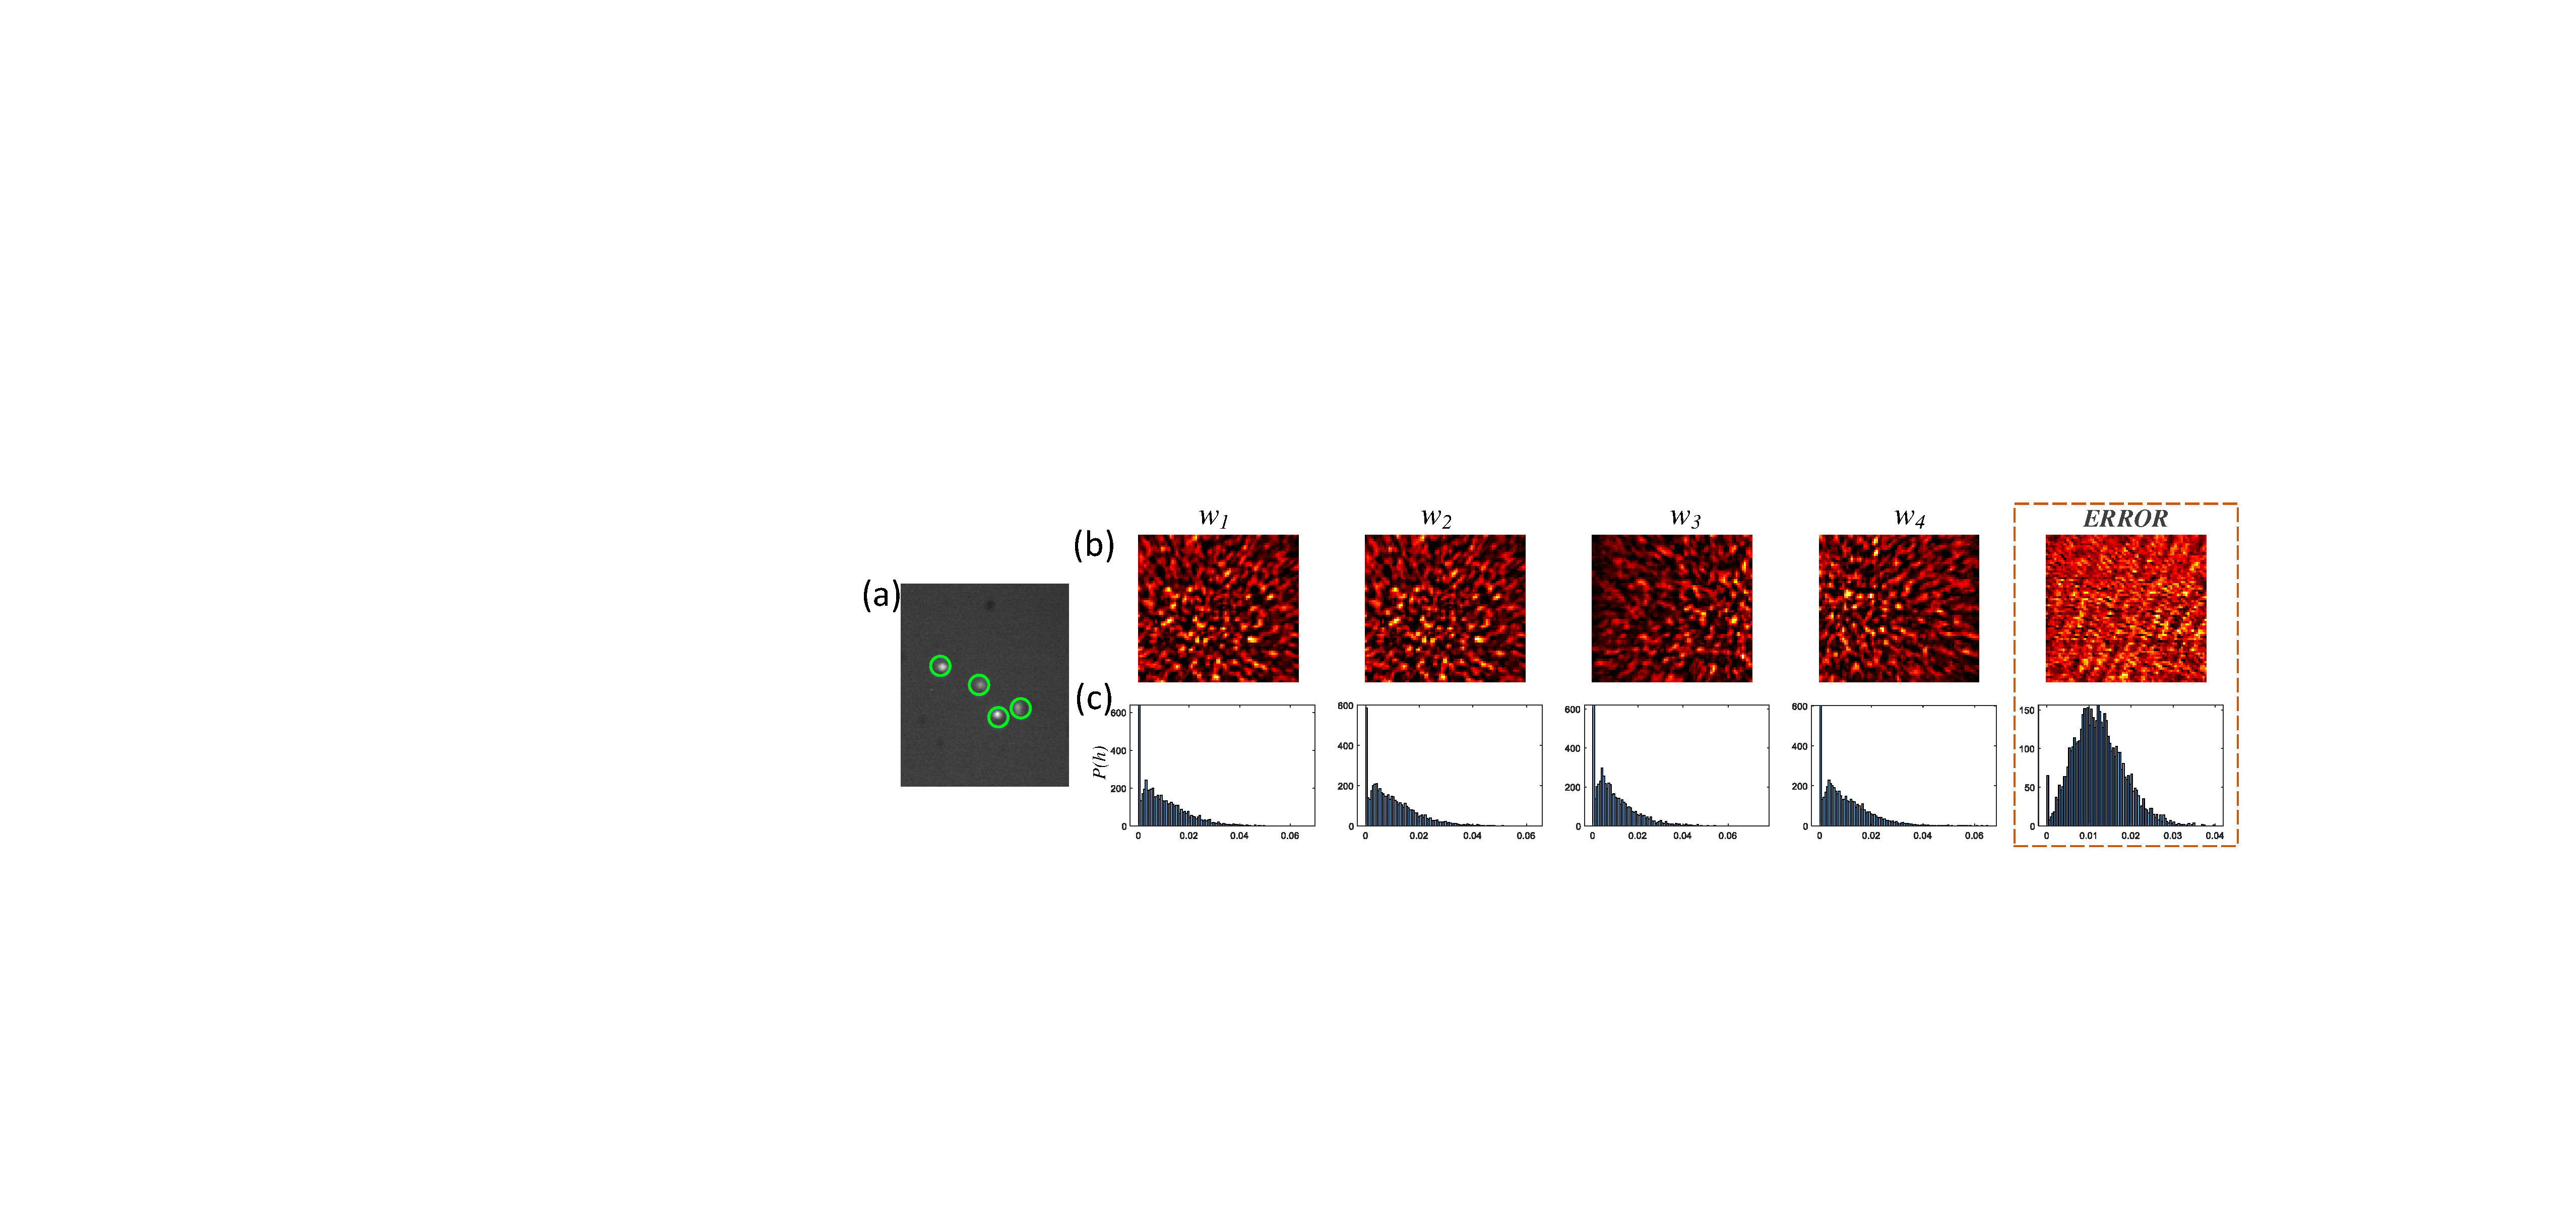
\includegraphics[scale=0.30]{C5.fig7}
	\caption{散斑去混叠实验结果}
	\label{fig:5.7}
\end{figure}

为了更加直观的显示散斑去混叠的结果,我们进行了另外一组实验,实验结果如图\ref{fig:5.7}所示。将一系列散斑图案$I$通过NMF算法,分解为矩阵$W$和$H$。图\ref{fig:5.7}(a)为原始目标,图\ref{fig:5.7}(b)为去混叠后散斑(来自于矩阵$W$)和图\ref{fig:5.7}(c)为对应图\ref{fig:5.7}(b)各自去混叠散斑的强度分布图。如图\ref{fig:5.7}中,虚线所标出的去混叠散斑,该散斑为算法所制造的噪声,当没有正确的估计数据集的秩可能造成此种结果。可以通过分析去混叠散斑的强度分布图进行剔除操作。但是,在本章所提出的重建方法中未使用此操作。

\subsubsection*{\textbf{\textit{NMF算法}}}

NMF的早期工作是由芬兰的一组研究人员\cite{paatero_positive_1994}在1990年代中期以正矩阵分解的方式进行的。 在 Lee 和 Seung 之后,它被广泛称为非负矩阵分解研究了NMF的两种不同分解算法的特性\cite{lee_learning_1999,lee_algorithms_2001}。它们仅在量化近似质量的成本函数上略有不同。一种算法可以最小化传统的最小二乘误差,而另一种算法最小化广义Kullback-Leibler散度。在这里,我们仅描述在去混叠过程中所使用的的传统最小二乘误差类型。为了找到近似的因式分解$I \approx WH$,一个简单的评价函数为度量是 $I$ 和 $WH$ 之间的欧几里得距离的平方,即对应于Frobenius范数:

\begin{equation}
	\begin{aligned}
\Arrowvert I -WH\Arrowvert_F^{2} = \sum_{i,j} (I -WH)_{i,j}^2,
\label{eq:5.3}
\end{aligned}
\end{equation}

虽然函数$\Arrowvert I -WH\Arrowvert_F^{2}$仅在$W$或仅$H$是凸的,它的两个变量$W$和$H$不同时为凸。因此,通过寻找全局最小值去解决此问题较难实现。然而,有许多数值优化技术可用于寻找局部最小值。交替成本的最小化导致了交替最小二乘法 (Alternating Least Squares,ALS) 算法:在这种方法中,在$W$和$H$的初始随机初始化之后,迭代地执行 $W$ 固定 $H$ 和 执行$H$ 固定 $W$ 的最小二乘解,直到成本函数达到最小值,或连续迭代之间的成本函数差异变得小于给定的容差值,或达到最大迭代次数。在每次迭代中,$W$和$H$ 的负元素被替换为$0$或很小的数。由于NMF算的稳定性和可解释性,该算法已经在众多领域有着较多的应用。
